\subsection{On-going Work on Neural Program Dependence Analysis}
\label{sec:deeppda}

In the neural network-based dependency parsing
approaches~\cite{chen-manning-2014-fast} in NLP, by projecting the
words into an embedding space, researchers successfully learn the
semantic relationships that model the dependencies between them. Thus
inspired, we believe we can follow suit to learn the control-flow and
program dependencies between the statements in programs as
well. Moreover, given that the quality of the statement embeddings
determines the accurate prediction of the program dependence
relations, enhancing them by incorporating context from both within
and across the statements is crucial. Intra-statement
contextualization can help relay the local information within
individual statements globally. For example, such information can help
distinguishably identify the declaration and reference of the same
variable across different program statements. In contrast,
inter-statement contextualization helps learn the dependencies between
the statements in the context of the surrounding statements. Finally,
we aim to model the CFG/PDG construction as a pairwise dependence
decoding task, wherein the combination of all the predicted edges in
the statement pairs can be formalized as directed graphs, i.e., a
program's CFG/PDG.

\begin{figure*}[ht]
\begin{center}
    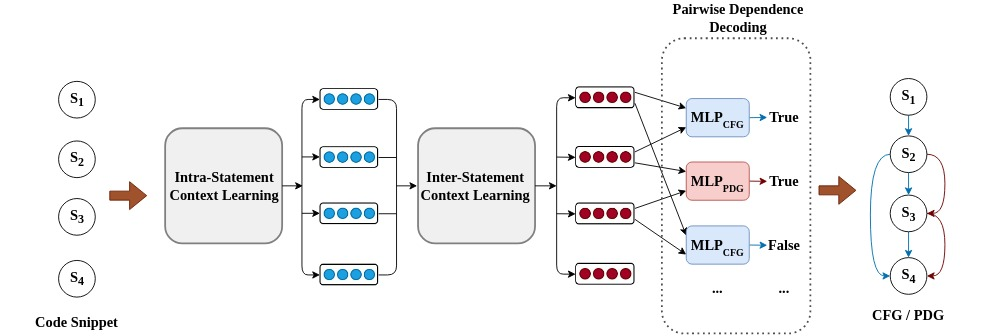
\includegraphics[width=0.9\textwidth]{model-abstract.jpg}
    \caption{Preliminary Design for \tool Model Infrastructure for Dependency Analysis for Partial Code}
    \label{fig:model}
    \vspace{-10pt}
\end{center}
\end{figure*}

In Figure~\ref{fig:model}, we present a preliminary design of the
general architecture of \tool model. Given that attention is the
driver behind the now ubiquitous Transformers’~\cite{Vaswani-2017}
success in efficiently learning representations for different entities
in different contexts, we plan to make it the foundation of the
context learning components in our model as well. Each is intended to
learn different aspects of contextualization.

%\begin{figure*}
%    \centering
%  \subfloat[Intra-Statement Context Learning\label{fig:input_repr_a}]{%
%       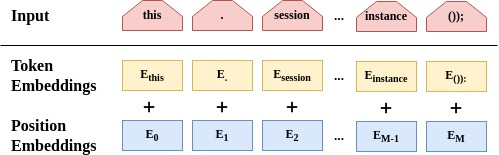
\includegraphics[width=0.45\linewidth]{figures/input_repr_tok.jpg}}
%  \hspace{0.25cm}
%  \subfloat[Inter-Statement Context Learning\label{fig:input_repr_b}]{%
%        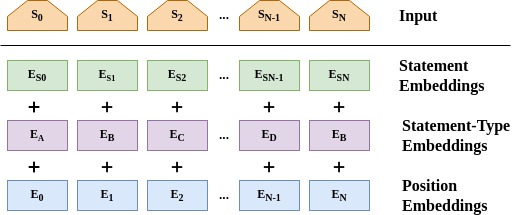
\includegraphics[width=0.45\linewidth]{figures/input_repr_stmt.jpg}}
%    \hfill
%  \caption{Input representations: (a) tokens in a statement are the sums of token embeddings, and (token) position embeddings; (b) statements in a snippet are the sums of statement embeddings, statement-type embeddings, and (statement) position~embeddings.}
%  \label{fig:input_repr}
%\end{figure*}


%\subsection{\bf Model Architecture}
%\label{sec:ppda_arch}

%As explained in Section~\ref{sec:overview}, better contextualization
%is the main idea behind \tool's design. Given that attention is the
%component in the ubiquitous Transformers'~\cite{Vaswani-2017} success
%in efficiently learning representations for different entities in
%different contexts, we chose to make it the foundation of our
%model. In brief, we realize \tool via a hierarchical, self-attention
%network (SAN)-based model architecture, where each sub-network is
%intended to capture different aspects of contextualization. Its
%details are as follows:

\vspace{2pt}
\subsubsection{{\bf Intra-Statement Context Learning (IntraS-CL)}}
\label{sec:ppda_arch_intra}
The syntactic and semantic knowledge of the code tokens within a
single statement must be made available globally to other statements
in a program to learn the inter-statement program dependencies
effectively. We enable this via a \textit{1-Layer} (i.e., $N_X$$=$$1$)
Self Attention Network (1L-SAN). The self-attention layer in an 1L-SAN
inputs $x_1, x_2, ..., x_n \in \mathbb{R}^d$, performs self-attention
once by projecting the inputs from all attention heads $\in
\mathbb{R}^{d_h}$ into the head dimension space $d_h$ via linear
transformations, and generate outputs $y_1, y_2, ..., y_n \in
\mathbb{R}^d$ which are linear combinations of the concatenated
attention head values. We use one attention head
(i.e., $h$$=$$1$) for the self-attention layer in 1L-SAN, and the size
of the input representations, i.e., $d$ is set to 512. Our experiments
revealed only a marginal performance gain by expanding the 1L-SAN to a
2L-SAN, which also came with high computational
overhead. Besides, increasing the number of attention heads did not
help either performance or interpretability. A more detailed analysis
on hyperparameters and subsequent
trade-offs is left to future~work.

\vspace{1pt} \underline{Input Representations}. For a program
comprising $N$ statements $s_1, s_2, ..., s_N$, \tool takes as input a
concatenation of $N$ sequences of $M$ tokens each, $\langle
t_1^{(1)}$, $t_2^{(1)}$.., $t_M^{(1)} \rangle$, ..., $\langle
t_1^{(N)}$, $t_2^{(N)}$.., $t_M^{(N)} \rangle$. Next, each token
sequence $\langle t_1^{(i)}$, $t_2^{(i)}$.., $t_M^{(i)} \rangle$ is
input to the 1L-SAN for intra-statement contextualization. Previous
works~\cite{radford2019language, liu2019roberta} have demonstrated
the~advantages of a byte-level Byte-Pair Encoding (BPE)-scheme for
tokenization. We follow suit to train a byte-level BPE tokenizer for
converting a given statement into a sequence of tokens. Here, $M$ is
the maximum number of tokens allowed in a statement.  For statements
with token sequences having ${<}M$ tokens, a special \textit{[PAD]}
token is appended. In contrast, token sequences having ${>}M$ tokens
are truncated to $M$ tokens.

%\vspace{1pt} \underline{Token Embeddings}. For all the words in the
%vocabulary $V$, we leverage a learnable embedding to learn and store
%their representations (i.e., $\mathbb{R}^{|V| \times d}$). Using this
%as a lookup table, token embeddings are retrieved for all the tokens
%generated by the tokenizer for a given statement.

%\vspace{1pt} \underline{Token Position Embeddings}. Attention
%mechanism in the self-attention layer is invariant to position
%information. However, this knowledge is key to understanding the
%sequential nature of code tokens in a statement. We enable this via
%learnable position encoding scheme, where a vector $\in \mathbb{R}^d$
%unique to each position is learned during the training process.

%\vspace{1pt} \underline{Statement (Output) Representations}. Input
%representations to the 1L-SAN corresponding to the tokens in a given
%statement are taken as the sums of the \textit{token embeddings}, and
%their \textit{position embeddings} (as in
%Fig.~\ref{fig:input_repr_a}). The 1L-SAN yields intra-statement
%contextualized token representations as its output, which are then
%averaged to retrieve the statement representation. Note that the token
%representations corresponding to the \textit{[PAD]} tokens are not
%considered for averaging. Such statement representations $u_i$ ($\in
%\mathbb{R}^d$) for all the statements $s_i \in s_1 ... s_N$ are then
%passed on for inter-statement contextualization.

\vspace{2pt}
\subsubsection{\bf Inter-Statement Context Learning (InterS-CL)}
The knowledge of surrounding statements in the context of a given
statement helps \tool model the dependencies between them better. We
enable this via a multi-layer bidirectional Transformer encoder based
on the work by Vaswani {\em et
  al.}~\cite{Vaswani-2017}. Owing to its common usage, we will omit
exhaustive background details on Transformers' model architecture and
will refer the readers to ~\cite{Vaswani-2017}. As shown in
Fig.~\ref{fig:model}, we denote the number of layers in the
Transformer encoder by $N_Y$, which we set to 6. We employ 4 attention
heads, i.e., $h$$=$$4$ to increase parallelization (since
$d_h$$=$$\frac{d}{h}$, i.e., $d_h$$=$$128$) and learn different
aspects of the syntactic and semantic structure in the statements,
while still being interpretable. We also set the feed-forward module
size to be 4 times that of the size of the input representations $d$,
i.e., 2048. Overall, Transformer in InterS-CL phase inputs
local context-aware statement representations $u_i \in \mathbb{R}^d$
for all statements $s_i$ in a given program, and outputs statement
representations $v_i \in \mathbb{R}^d$ that are both local and global
context-aware.

\vspace{1pt} \underline{Statement Input Representations}. For all the
statements $s_i$, statement embeddings (i.e., $u_i \in
\mathbb{R}^d$) are obtained from the 1L-SAN in the IntraS-CL phase.
$N$ is the maximum number of statements in a method in the dataset. If
a given program has less than $N$ statements,
zero vectors ($\in \mathbb{R}^d$) are padded to the inputs.

%\vspace{1pt} \underline{Statement Position Embeddings}. To make our
%model under\-stand the sequential nature of statements in a program,
%as~in Section~\ref{sec:ppda_arch_intra}, we leverage a learnable
%position encoding~sch\-eme to learn unique vectors ($\in
%\mathbb{R}^d$) for all statement~positions.

%\vspace{1pt} \underline{Statement Types}. Most neural network-based
%dependency parsers leverage parts-of-speech (POS) tags for the words
%in a sentence for better dependency learning. Thus inspired, we chose
%to associate with each statement a label indicating the
%\textit{statement type}, which is essentially the type of the AST node
%rooted at the sub-AST for the statement. We extract labels such as
%\code{METHOD}, \code{CONTROL\_STRUCTURE}, \code{BLOCK}, etc., which
%helps augment the statement with such syntactic information. We learn
%unique vectors ($\in \mathbb{R}^d$) for each of the statement types.

%\vspace{1pt} \underline{Statement (Output) Representations}. As shown
%in Fig.~\ref{fig:input_repr_b}, the input representations for the
%statements in a program are taken as the sums of the \textit{statement
%  embeddings}, \textit{statement-type embeddings}, and the
%\textit{statement position embeddings}. These are then passed on to
%the Transformer encoder, to retrieve contextualized statement representations $v_i
%\in \mathbb{R}^d$ for all the statements $s_i \in s_1 ... s_N$, that model
%the syntactic and semantic knowledge from both within and across the
%statements. After this, we obtain the contextualized statement representations.

\vspace{1pt}
\subsubsection{\bf Pairwise Dependence Decoding}
%Pairs of latent feature vectors $\langle v_i, v_j \rangle$ (1$\leq i, j\leq$ N) are taken from the sequence of intra and inter-statement contextualized statement representations corresponding to all statements in a program, to detect the presence of CFG/PDG edges between them. A combination of all such CFG/PDG edges extracted via the arc-factored approach is realized as the CFG/PDG for the given program. We leverage 2-layered multi-layer perceptron networks (one each for detecting CFG and PDG edges, i.e., MLP\textsubscript{CFG} and MLP\textsubscript{PDG} respectively) for the pairwise dependence decoding phase, which are scored as follows:

From the sequence of contextualized statement representations $v_i \in
\mathbb{R}^d$ corresponding to all the statements in a program passed
on by the Transformer encoder in the InterS-CL phase, pairs such
as $\langle v_i, v_j \rangle$ (1$\leq i, j\leq$ N) are taken to detect
the presence of CFG/PDG edges between two statements $s_i$ and
$s_j$. We leverage 2-layered multi-layer perceptron networks (each
for detecting the CFG and PDG edges, i.e., MLP\textsubscript{CFG} and
MLP\textsubscript{PDG}, respectively) in the pairwise dependence
decoding phase, which are scored as follows:
\begin{equation}
\centering
    score\textsubscript{rel}(i, j) = MLP\textsubscript{rel}(v_i \circ v_j \circ (v_i * v_j) \circ |v_i - v_j|)
\end{equation}
where $\circ$, $*$ and $|.|$ correspond to concatenation, element-wise
product, and absolute element-wise difference operations respectively;
and \textit{rel} represents either the control-flow or program
dependence relations. Attaining a $score\textsubscript{rel}(i, j) >
0.5$ represents the detection of the corresponding CFG/PDG edge from
statement $s_i$ to statement $s_j$. The combination of all the CFG/PDG
edges extracted via such an arc-factored approach is realized as the
CFG/PDG for the given program.

\subsubsection{\bf Training Process}

Training \tool requires the knowledge of ground-truth CFG and PDG edges between statements in a program. Thus, it can only be trained on complete programs (at a minimum, which are at a method-level granularity) so as to be able to leverage program analysis tools to extract them. The CFG and PDG edge information can then be utilized to compute the training objective loss (i.e., $\mathcal{L}$) for our model as follows: $\mathcal{L} = \mathcal{L}\textsubscript{CFG} + \mathcal{L}\textsubscript{PDG}$
%\begin{equation}
%    \centering
%    $$\mathcal{L} = \mathcal{L}\textsubscript{CFG} + \mathcal{L}\textsubscript{PDG}$$
%\end{equation}
where $\mathcal{L}\textsubscript{CFG}$ is the loss for CFG edge-decoding, and $\mathcal{L}\textsubscript{PDG}$ is the loss for PDG edge-decoding. Moreover, $\mathcal{L}\textsubscript{CFG}$ and $\mathcal{L}\textsubscript{PDG}$ are computed as the sums of all binary-cross entropy (BCE) losses corresponding to the CFG and PDG edge predictions between different statements in a program. Note that the inter-statement losses corresponding to the edges from/to the zero-padded statements do not contribute to either $\mathcal{L}\textsubscript{CFG}$ or $\mathcal{L}\textsubscript{PDG}$. The model parameters which are learned to minimize $\mathcal{L}$ include learnable embeddings (token, token position, statement type, and statement position), attention, Tr-FFNN (i.e., feed-forward neural network in Transformer encoder), MLP\textsubscript{CFG}, and MLP\textsubscript{PDG}.

%Overall, \tool has about 39M parameters.

\subsubsection{\bf Inference for Dependency Discovery}
\label{sec:inference}
Despite being trained on only complete code, one can leverage \tool to extract the control-flow and program dependence edges for both complete and partial code. The following, however, are the important points of consideration:
%\textit{Statement Types}: To extract the syntactic information encoded
%in \textit{statement types}, one would need the program's AST. In
%Java, for example, this can be retrieved even if the code is
%incomplete using tools such as PPA~\cite{dagenais-2008}. However, this
%is not possible for all programming languages. In such cases, \tool
%can be trained without statement types, i.e., by computing the input
%representation for statements in a program as just the sums of the
%statement and their position embeddings. In
%Section~\ref{sec:ablation}, we demonstrate the practicality of such an
%alternative.
\textit{Programs with ${\leq}N$ statements}: Making use of a trained
\tool model on both complete and partial programs, the number of
statements in which is less than the \textit{maximum statements}
allowed in the model is straightforward. In such cases, \tool predicts
the CFG/PDG edges from one statement to another by contextualizing
over all the other statements in the program.
\textit{Programs with ${>}N$ statements}: For (both complete and
partial) programs having number of statements greater than that
allowed in the trained \tool model, we have the following strategies
in {\tool}: (a) train a model with a higher value of $N$, (b) chunk
the program into $N$-statement code fragments, predict CFG/PDG edges
for each of the code fragments independently, and finally, combine the
CFG/PDG predictions for all the fragments. For example, if a trained
model allows a maximum of 16 statements, to predict for a program with
46 statements, one can break it down into code fragments with 16, 16,
and 14 statements, respectively.

%A potential downside to strategy (b), however, is that a statement in
%a fragment will be contextualized only over the other statements in
%that fragment, and the control-flow and program dependencies across
%fragments will not be captured. Increasing $N$ could address this
%issue, albeit with more computational overhead.

%\end{itemize}
